\documentclass[1p]{elsarticle_modified}
%\bibliographystyle{elsarticle-num}

%\usepackage[colorlinks]{hyperref}
%\usepackage{abbrmath_seonhwa} %\Abb, \Ascr, \Acal ,\Abf, \Afrak
\usepackage{amsfonts}
\usepackage{amssymb}
\usepackage{amsmath}
\usepackage{amsthm}
\usepackage{scalefnt}
\usepackage{amsbsy}
\usepackage{kotex}
\usepackage{caption}
\usepackage{subfig}
\usepackage{color}
\usepackage{graphicx}
\usepackage{xcolor} %% white, black, red, green, blue, cyan, magenta, yellow
\usepackage{float}
\usepackage{setspace}
\usepackage{hyperref}

\usepackage{tikz}
\usetikzlibrary{arrows}

\usepackage{multirow}
\usepackage{array} % fixed length table
\usepackage{hhline}

%%%%%%%%%%%%%%%%%%%%%
\makeatletter
\renewcommand*\env@matrix[1][\arraystretch]{%
	\edef\arraystretch{#1}%
	\hskip -\arraycolsep
	\let\@ifnextchar\new@ifnextchar
	\array{*\c@MaxMatrixCols c}}
\makeatother %https://tex.stackexchange.com/questions/14071/how-can-i-increase-the-line-spacing-in-a-matrix
%%%%%%%%%%%%%%%

\usepackage[normalem]{ulem}

\newcommand{\msout}[1]{\ifmmode\text{\sout{\ensuremath{#1}}}\else\sout{#1}\fi}
%SOURCE: \msout is \stkout macro in https://tex.stackexchange.com/questions/20609/strikeout-in-math-mode

\newcommand{\cancel}[1]{
	\ifmmode
	{\color{red}\msout{#1}}
	\else
	{\color{red}\sout{#1}}
	\fi
}

\newcommand{\add}[1]{
	{\color{blue}\uwave{#1}}
}

\newcommand{\replace}[2]{
	\ifmmode
	{\color{red}\msout{#1}}{\color{blue}\uwave{#2}}
	\else
	{\color{red}\sout{#1}}{\color{blue}\uwave{#2}}
	\fi
}

\newcommand{\Sol}{\mathcal{S}} %segment
\newcommand{\D}{D} %diagram
\newcommand{\A}{\mathcal{A}} %arc


%%%%%%%%%%%%%%%%%%%%%%%%%%%%%5 test

\def\sl{\operatorname{\textup{SL}}(2,\Cbb)}
\def\psl{\operatorname{\textup{PSL}}(2,\Cbb)}
\def\quan{\mkern 1mu \triangleright \mkern 1mu}

\theoremstyle{definition}
\newtheorem{thm}{Theorem}[section]
\newtheorem{prop}[thm]{Proposition}
\newtheorem{lem}[thm]{Lemma}
\newtheorem{ques}[thm]{Question}
\newtheorem{cor}[thm]{Corollary}
\newtheorem{defn}[thm]{Definition}
\newtheorem{exam}[thm]{Example}
\newtheorem{rmk}[thm]{Remark}
\newtheorem{alg}[thm]{Algorithm}

\newcommand{\I}{\sqrt{-1}}
\begin{document}

%\begin{frontmatter}
%
%\title{Boundary parabolic representations of knots up to 8 crossings}
%
%%% Group authors per affiliation:
%\author{Yunhi Cho} 
%\address{Department of Mathematics, University of Seoul, Seoul, Korea}
%\ead{yhcho@uos.ac.kr}
%
%
%\author{Seonhwa Kim} %\fnref{s_kim}}
%\address{Center for Geometry and Physics, Institute for Basic Science, Pohang, 37673, Korea}
%\ead{ryeona17@ibs.re.kr}
%
%\author{Hyuk Kim}
%\address{Department of Mathematical Sciences, Seoul National University, Seoul 08826, Korea}
%\ead{hyukkim@snu.ac.kr}
%
%\author{Seokbeom Yoon}
%\address{Department of Mathematical Sciences, Seoul National University, Seoul, 08826,  Korea}
%\ead{sbyoon15@snu.ac.kr}
%
%\begin{abstract}
%We find all boundary parabolic representation of knots up to 8 crossings.
%
%\end{abstract}
%\begin{keyword}
%    \MSC[2010] 57M25 
%\end{keyword}
%
%\end{frontmatter}

%\linenumbers
%\tableofcontents
%
\newcommand\colored[1]{\textcolor{white}{\rule[-0.35ex]{0.8em}{1.4ex}}\kern-0.8em\color{red} #1}%
%\newcommand\colored[1]{\textcolor{white}{ #1}\kern-2.17ex	\textcolor{white}{ #1}\kern-1.81ex	\textcolor{white}{ #1}\kern-2.15ex\color{red}#1	}

{\Large $\underline{10_{162}~(K10n_{40})}$}

\setlength{\tabcolsep}{10pt}
\renewcommand{\arraystretch}{1.6}
\vspace{1cm}\begin{tabular}{m{100pt}>{\centering\arraybackslash}m{274pt}}
\multirow{5}{120pt}{
	\centering
	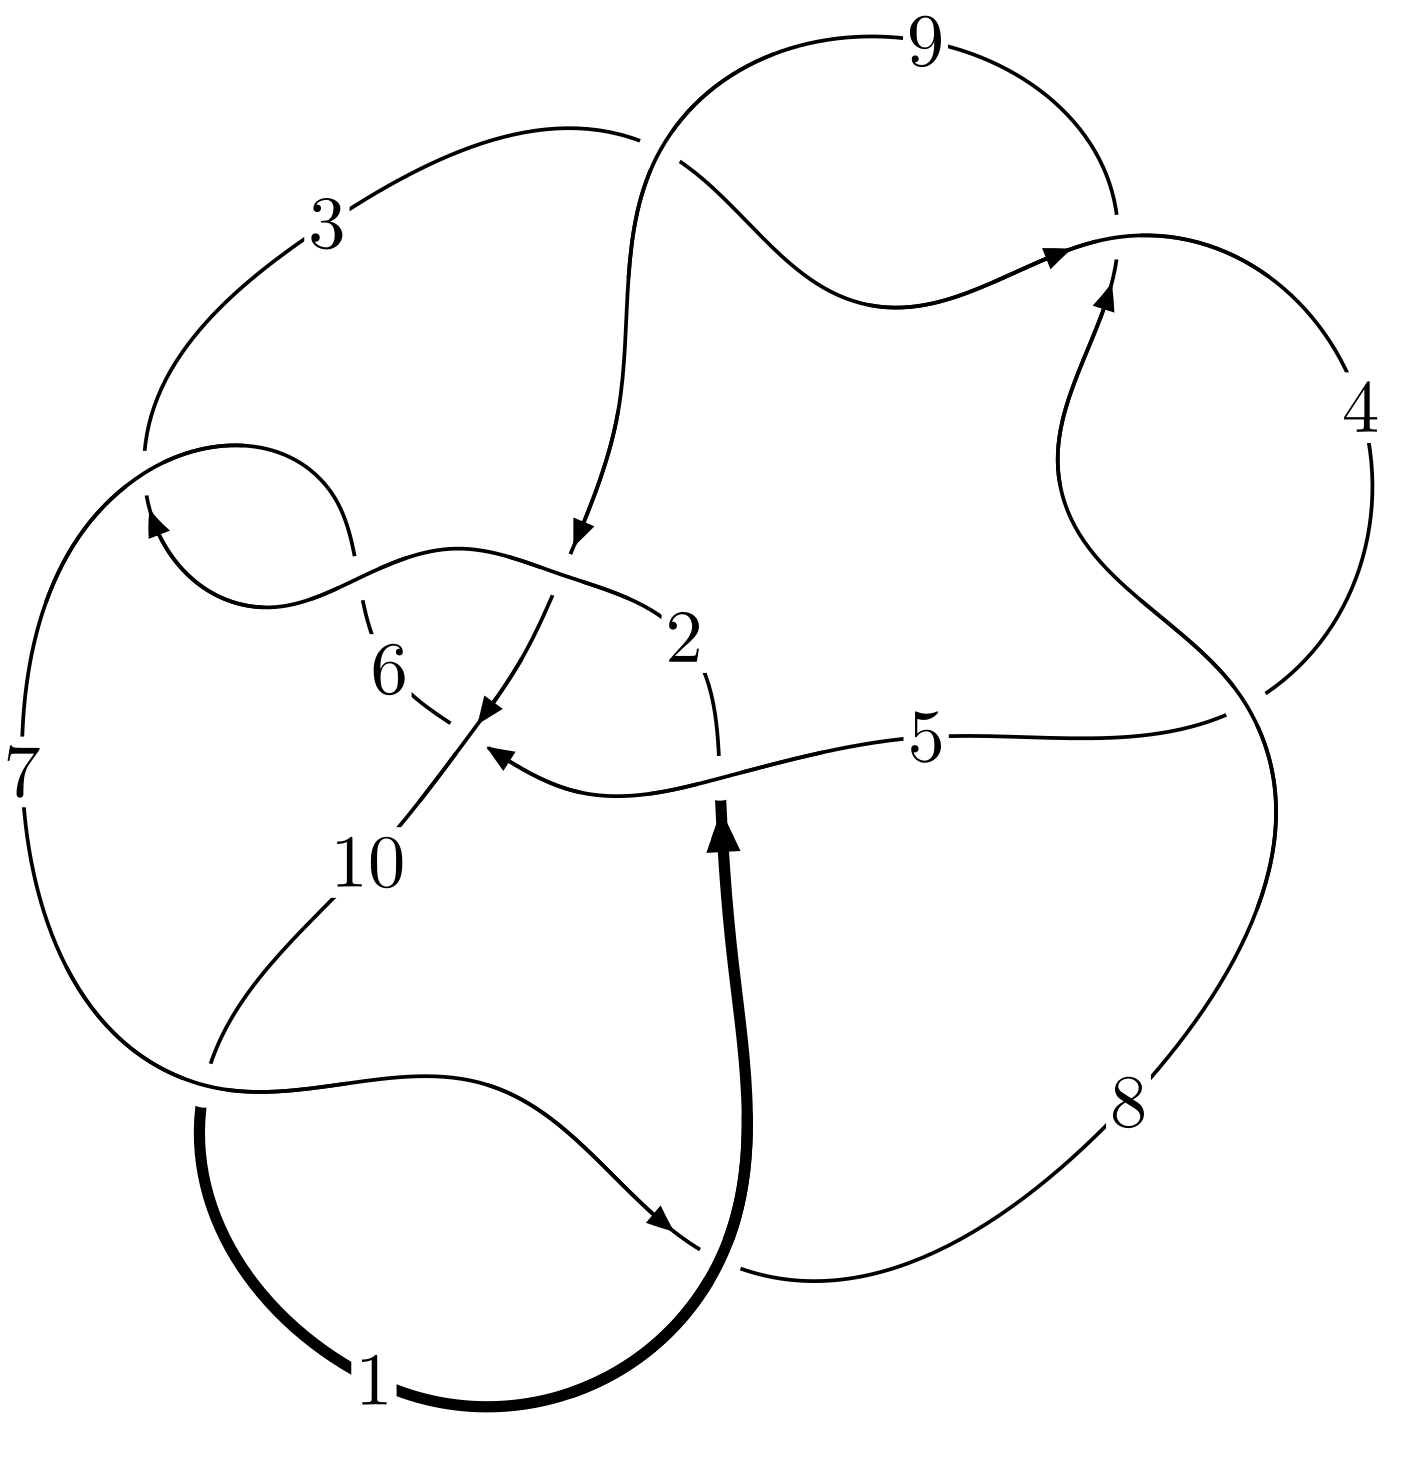
\includegraphics[width=112pt]{../../../GIT/diagram.site/Diagrams/png/246_10_162.png}\\
\ \ \ A knot diagram\footnotemark}&
\allowdisplaybreaks
\textbf{Linearized knot diagam} \\
\cline{2-2}
 &
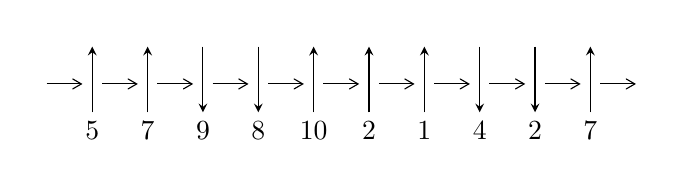
\begin{tikzpicture}[x=20pt, y=17pt]
	% nodes
	\node (C0) at (0, 0) {};
	\node (C1) at (1, 0) {};
	\node (C1U) at (1, +1) {};
	\node (C1D) at (1, -1) {5};

	\node (C2) at (2, 0) {};
	\node (C2U) at (2, +1) {};
	\node (C2D) at (2, -1) {7};

	\node (C3) at (3, 0) {};
	\node (C3U) at (3, +1) {};
	\node (C3D) at (3, -1) {9};

	\node (C4) at (4, 0) {};
	\node (C4U) at (4, +1) {};
	\node (C4D) at (4, -1) {8};

	\node (C5) at (5, 0) {};
	\node (C5U) at (5, +1) {};
	\node (C5D) at (5, -1) {10};

	\node (C6) at (6, 0) {};
	\node (C6U) at (6, +1) {};
	\node (C6D) at (6, -1) {2};

	\node (C7) at (7, 0) {};
	\node (C7U) at (7, +1) {};
	\node (C7D) at (7, -1) {1};

	\node (C8) at (8, 0) {};
	\node (C8U) at (8, +1) {};
	\node (C8D) at (8, -1) {4};

	\node (C9) at (9, 0) {};
	\node (C9U) at (9, +1) {};
	\node (C9D) at (9, -1) {2};

	\node (C10) at (10, 0) {};
	\node (C10U) at (10, +1) {};
	\node (C10D) at (10, -1) {7};
	\node (C11) at (11, 0) {};

	% arrows
	\draw[->,>={angle 60}]
	(C0) edge (C1) (C1) edge (C2) (C2) edge (C3) (C3) edge (C4) (C4) edge (C5) (C5) edge (C6) (C6) edge (C7) (C7) edge (C8) (C8) edge (C9) (C9) edge (C10) (C10) edge (C11) ;	\draw[->,>=stealth]
	(C1D) edge (C1U) (C2D) edge (C2U) (C3U) edge (C3D) (C4U) edge (C4D) (C5D) edge (C5U) (C6D) edge (C6U) (C7D) edge (C7U) (C8U) edge (C8D) (C9U) edge (C9D) (C10D) edge (C10U) ;
	\end{tikzpicture} \\
\hhline{~~} \\& 
\textbf{Solving Sequence} \\ \cline{2-2} 
 &
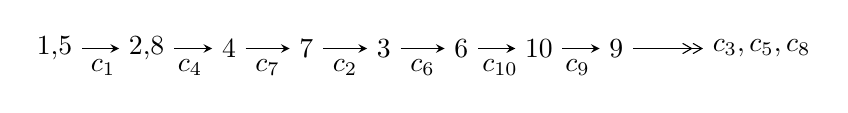
\begin{tikzpicture}[x=28pt, y=7pt]
	% node
	\node (A0) at (-1/8, 0) {1,5};
	\node (A1) at (17/16, 0) {2,8};
	\node (A2) at (17/8, 0) {4};
	\node (A3) at (25/8, 0) {7};
	\node (A4) at (33/8, 0) {3};
	\node (A5) at (41/8, 0) {6};
	\node (A6) at (49/8, 0) {10};
	\node (A7) at (57/8, 0) {9};
	\node (C1) at (1/2, -1) {$c_{1}$};
	\node (C2) at (13/8, -1) {$c_{4}$};
	\node (C3) at (21/8, -1) {$c_{7}$};
	\node (C4) at (29/8, -1) {$c_{2}$};
	\node (C5) at (37/8, -1) {$c_{6}$};
	\node (C6) at (45/8, -1) {$c_{10}$};
	\node (C7) at (53/8, -1) {$c_{9}$};
	\node (A8) at (9, 0) {$c_{3},c_{5},c_{8}$};

	% edge
	\draw[->,>=stealth]	
	(A0) edge (A1) (A1) edge (A2) (A2) edge (A3) (A3) edge (A4) (A4) edge (A5) (A5) edge (A6) (A6) edge (A7) ;
	\draw[->>,>={angle 60}]	
	(A7) edge (A8);
\end{tikzpicture} \\ 

\end{tabular} \\

\footnotetext{
The image of knot diagram is generated by the software ``\textbf{Draw programme}" developed by Andrew Bartholomew(\url{http://www.layer8.co.uk/maths/draw/index.htm\#Running-draw}), where we modified some parts for our purpose(\url{https://github.com/CATsTAILs/LinksPainter}).
}\phantom \\ \newline 
\centering \textbf{Ideals for irreducible components\footnotemark of $X_{\text{par}}$} 
 
\begin{align*}
I^u_{1}&=\langle 
b- u,\;- u^9+u^8+3 u^7-2 u^6-8 u^5+3 u^4+8 u^3+a-5 u+2,\\
\phantom{I^u_{1}}&\phantom{= \langle  }u^{10}- u^9-3 u^8+3 u^7+7 u^6-5 u^5-6 u^4+4 u^3+3 u^2-3 u+1\rangle \\
I^u_{2}&=\langle 
-30 u^{11}+6 u^{10}+76 u^9-92 u^8+34 u^7+209 u^6-204 u^5-228 u^4+66 u^3+529 u^2+95 b+28 u-416,\\
\phantom{I^u_{2}}&\phantom{= \langle  }-336 u^{11}+50 u^{10}+\cdots+1045 a-3305,\\
\phantom{I^u_{2}}&\phantom{= \langle  }u^{12}- u^{11}-2 u^{10}+5 u^9-4 u^8-5 u^7+11 u^6+u^5-6 u^4-16 u^3+16 u^2+10 u-11\rangle \\
I^u_{3}&=\langle 
b+u,\;u^2+a-1,\;u^5- u^4- u^3+u^2+1\rangle \\
\\
\end{align*}
\raggedright * 3 irreducible components of $\dim_{\mathbb{C}}=0$, with total 27 representations.\\
\footnotetext{All coefficients of polynomials are rational numbers. But the coefficients are sometimes approximated in decimal forms when there is not enough margin.}
\newpage
\renewcommand{\arraystretch}{1}
\centering \section*{I. $I^u_{1}= \langle b- u,\;- u^9+u^8+\cdots+a+2,\;u^{10}- u^9+\cdots-3 u+1 \rangle$}
\flushleft \textbf{(i) Arc colorings}\\
\begin{tabular}{m{7pt} m{180pt} m{7pt} m{180pt} }
\flushright $a_{1}=$&$\begin{pmatrix}1\\0\end{pmatrix}$ \\
\flushright $a_{5}=$&$\begin{pmatrix}0\\u\end{pmatrix}$ \\
\flushright $a_{2}=$&$\begin{pmatrix}1\\- u^2\end{pmatrix}$ \\
\flushright $a_{8}=$&$\begin{pmatrix}u^9- u^8-3 u^7+2 u^6+8 u^5-3 u^4-8 u^3+5 u-2\\u\end{pmatrix}$ \\
\flushright $a_{4}=$&$\begin{pmatrix}u^9- u^8-2 u^7+3 u^6+3 u^5-3 u^4+u^3+3 u^2-2 u\\- u^8+u^7+2 u^6-2 u^5-4 u^4+2 u^3+u^2\end{pmatrix}$ \\
\flushright $a_{7}=$&$\begin{pmatrix}u^9- u^8-3 u^7+2 u^6+8 u^5-3 u^4-8 u^3+4 u-2\\u\end{pmatrix}$ \\
\flushright $a_{3}=$&$\begin{pmatrix}-2 u^9+u^8+5 u^7- u^6-12 u^5-2 u^4+7 u^3+2 u^2-4 u+3\\u^9- u^8-2 u^7+2 u^6+4 u^5- u^4- u^3- u^2\end{pmatrix}$ \\
\flushright $a_{6}=$&$\begin{pmatrix}u^9-4 u^7+10 u^5+u^4-9 u^3- u^2+4 u-2\\- u^8+u^7+3 u^6-4 u^5-5 u^4+4 u^3+3 u^2-2 u+1\end{pmatrix}$ \\
\flushright $a_{10}=$&$\begin{pmatrix}- u^7+u^6+2 u^5-2 u^4-4 u^3+u^2+u\\u^2\end{pmatrix}$ \\
\flushright $a_{9}=$&$\begin{pmatrix}- u^9+u^8+u^7- u^6-2 u^5- u^4-3 u^3+2 u^2+u\\u^9- u^8-3 u^7+4 u^6+5 u^5-5 u^4-3 u^3+4 u^2- u\end{pmatrix}$\\&\end{tabular}
\flushleft \textbf{(ii) Obstruction class $= -1$}\\~\\
\flushleft \textbf{(iii) Cusp Shapes $= -5 u^9+4 u^8+16 u^7-11 u^6-39 u^5+15 u^4+38 u^3-11 u^2-21 u+14$}\\~\\
\newpage\renewcommand{\arraystretch}{1}
\flushleft \textbf{(iv) u-Polynomials at the component}\newline \\
\begin{tabular}{m{50pt}|m{274pt}}
Crossings & \hspace{64pt}u-Polynomials at each crossing \\
\hline $$\begin{aligned}c_{1},c_{7},c_{10}\end{aligned}$$&$\begin{aligned}
&u^{10}- u^9-3 u^8+3 u^7+7 u^6-5 u^5-6 u^4+4 u^3+3 u^2-3 u+1
\end{aligned}$\\
\hline $$\begin{aligned}c_{2},c_{5},c_{6}\end{aligned}$$&$\begin{aligned}
&u^{10}+7 u^8- u^7+20 u^6-6 u^5+25 u^4-8 u^3+10 u^2-2 u+1
\end{aligned}$\\
\hline $$\begin{aligned}c_{3},c_{4},c_{8}\end{aligned}$$&$\begin{aligned}
&u^{10}+5 u^9+\cdots+18 u+4
\end{aligned}$\\
\hline $$\begin{aligned}c_{9}\end{aligned}$$&$\begin{aligned}
&u^{10}-9 u^9+\cdots-20 u+8
\end{aligned}$\\
\hline
\end{tabular}\\~\\
\newpage\renewcommand{\arraystretch}{1}
\flushleft \textbf{(v) Riley Polynomials at the component}\newline \\
\begin{tabular}{m{50pt}|m{274pt}}
Crossings & \hspace{64pt}Riley Polynomials at each crossing \\
\hline $$\begin{aligned}c_{1},c_{7},c_{10}\end{aligned}$$&$\begin{aligned}
&y^{10}-7 y^9+\cdots-3 y+1
\end{aligned}$\\
\hline $$\begin{aligned}c_{2},c_{5},c_{6}\end{aligned}$$&$\begin{aligned}
&y^{10}+14 y^9+\cdots+16 y+1
\end{aligned}$\\
\hline $$\begin{aligned}c_{3},c_{4},c_{8}\end{aligned}$$&$\begin{aligned}
&y^{10}+9 y^9+\cdots+68 y+16
\end{aligned}$\\
\hline $$\begin{aligned}c_{9}\end{aligned}$$&$\begin{aligned}
&y^{10}-5 y^9+\cdots+496 y+64
\end{aligned}$\\
\hline
\end{tabular}\\~\\
\newpage\flushleft \textbf{(vi) Complex Volumes and Cusp Shapes}
$$\begin{array}{c|c|c}  
\text{Solutions to }I^u_{1}& \I (\text{vol} + \sqrt{-1}CS) & \text{Cusp shape}\\
 \hline 
\begin{aligned}
u &= \phantom{-}0.834890 + 0.288236 I \\
a &= -1.16719 - 0.85231 I \\
b &= \phantom{-}0.834890 + 0.288236 I\end{aligned}
 & -1.336140 - 0.440636 I & \phantom{-}5.86082 - 0.80149 I \\ \hline\begin{aligned}
u &= \phantom{-}0.834890 - 0.288236 I \\
a &= -1.16719 + 0.85231 I \\
b &= \phantom{-}0.834890 - 0.288236 I\end{aligned}
 & -1.336140 + 0.440636 I & \phantom{-}5.86082 + 0.80149 I \\ \hline\begin{aligned}
u &= -0.989389 + 0.553558 I \\
a &= -0.604538 + 1.276350 I \\
b &= -0.989389 + 0.553558 I\end{aligned}
 & \phantom{-}7.86026 - 2.34852 I & \phantom{-}3.25800 + 2.98056 I \\ \hline\begin{aligned}
u &= -0.989389 - 0.553558 I \\
a &= -0.604538 - 1.276350 I \\
b &= -0.989389 - 0.553558 I\end{aligned}
 & \phantom{-}7.86026 + 2.34852 I & \phantom{-}3.25800 - 2.98056 I \\ \hline\begin{aligned}
u &= -1.093020 + 0.614392 I \\
a &= \phantom{-}0.571463 + 0.630872 I \\
b &= -1.093020 + 0.614392 I\end{aligned}
 & -3.41629 - 5.60135 I & \phantom{-}2.31471 + 5.03009 I \\ \hline\begin{aligned}
u &= -1.093020 - 0.614392 I \\
a &= \phantom{-}0.571463 - 0.630872 I \\
b &= -1.093020 - 0.614392 I\end{aligned}
 & -3.41629 + 5.60135 I & \phantom{-}2.31471 - 5.03009 I \\ \hline\begin{aligned}
u &= \phantom{-}0.329249 + 0.368284 I \\
a &= \phantom{-}0.479615 + 1.097570 I \\
b &= \phantom{-}0.329249 + 0.368284 I\end{aligned}
 & \phantom{-}0.201388 + 1.011140 I & \phantom{-}3.39938 - 6.83831 I \\ \hline\begin{aligned}
u &= \phantom{-}0.329249 - 0.368284 I \\
a &= \phantom{-}0.479615 - 1.097570 I \\
b &= \phantom{-}0.329249 - 0.368284 I\end{aligned}
 & \phantom{-}0.201388 - 1.011140 I & \phantom{-}3.39938 + 6.83831 I \\ \hline\begin{aligned}
u &= \phantom{-}1.41827 + 0.76674 I \\
a &= \phantom{-}0.220652 + 0.935375 I \\
b &= \phantom{-}1.41827 + 0.76674 I\end{aligned}
 & \phantom{-}2.44804 + 10.69340 I & \phantom{-}5.16708 - 5.74333 I \\ \hline\begin{aligned}
u &= \phantom{-}1.41827 - 0.76674 I \\
a &= \phantom{-}0.220652 - 0.935375 I \\
b &= \phantom{-}1.41827 - 0.76674 I\end{aligned}
 & \phantom{-}2.44804 - 10.69340 I & \phantom{-}5.16708 + 5.74333 I\\
 \hline 
 \end{array}$$\newpage\newpage\renewcommand{\arraystretch}{1}
\centering \section*{II. $I^u_{2}= \langle -30 u^{11}+6 u^{10}+\cdots+95 b-416,\;-336 u^{11}+50 u^{10}+\cdots+1045 a-3305,\;u^{12}- u^{11}+\cdots+10 u-11 \rangle$}
\flushleft \textbf{(i) Arc colorings}\\
\begin{tabular}{m{7pt} m{180pt} m{7pt} m{180pt} }
\flushright $a_{1}=$&$\begin{pmatrix}1\\0\end{pmatrix}$ \\
\flushright $a_{5}=$&$\begin{pmatrix}0\\u\end{pmatrix}$ \\
\flushright $a_{2}=$&$\begin{pmatrix}1\\- u^2\end{pmatrix}$ \\
\flushright $a_{8}=$&$\begin{pmatrix}0.321531 u^{11}-0.0478469 u^{10}+\cdots+0.449761 u+3.16268\\0.315789 u^{11}-0.0631579 u^{10}+\cdots-0.294737 u+4.37895\end{pmatrix}$ \\
\flushright $a_{4}=$&$\begin{pmatrix}0.107177 u^{11}+0.0612440 u^{10}+\cdots-1.03254 u-0.359809\\0.284211 u^{11}+0.126316 u^{10}+\cdots-u+1.53684\end{pmatrix}$ \\
\flushright $a_{7}=$&$\begin{pmatrix}0.00574163 u^{11}+0.0153110 u^{10}+\cdots+0.744498 u-1.21627\\0.315789 u^{11}-0.0631579 u^{10}+\cdots-0.294737 u+4.37895\end{pmatrix}$ \\
\flushright $a_{3}=$&$\begin{pmatrix}0.123445 u^{11}-0.0181818 u^{10}+\cdots+0.0277512 u+2.61340\\-0.0210526 u^{11}-0.147368 u^{10}+\cdots+1.27368 u+0.936842\end{pmatrix}$ \\
\flushright $a_{6}=$&$\begin{pmatrix}-0.478469 u^{11}-0.00574163 u^{10}+\cdots+1.18660 u-5.82679\\\frac{4}{5} u^{11}-\frac{1}{19} u^{10}+\cdots-\frac{2}{95} u+\frac{944}{95}\end{pmatrix}$ \\
\flushright $a_{10}=$&$\begin{pmatrix}-0.144498 u^{11}-0.129187 u^{10}+\cdots+1.24593 u-1.67656\\0.284211 u^{11}+0.273684 u^{10}+\cdots-2.42105 u+2.07368\end{pmatrix}$ \\
\flushright $a_{9}=$&$\begin{pmatrix}-0.123445 u^{11}+0.0181818 u^{10}+\cdots-0.0277512 u-2.61340\\0.0315789 u^{11}+0.126316 u^{10}+\cdots-0.968421 u+0.221053\end{pmatrix}$\\&\end{tabular}
\flushleft \textbf{(ii) Obstruction class $= -1$}\\~\\
\flushleft \textbf{(iii) Cusp Shapes $= \frac{8}{19} u^{11}-\frac{36}{95} u^{10}-\frac{88}{95} u^9+\frac{32}{19} u^8-\frac{128}{95} u^7-\frac{44}{19} u^6+\frac{68}{19} u^5+\frac{8}{5} u^4-\frac{316}{95} u^3-\frac{148}{19} u^2+\frac{524}{95} u+\frac{706}{95}$}\\~\\
\newpage\renewcommand{\arraystretch}{1}
\flushleft \textbf{(iv) u-Polynomials at the component}\newline \\
\begin{tabular}{m{50pt}|m{274pt}}
Crossings & \hspace{64pt}u-Polynomials at each crossing \\
\hline $$\begin{aligned}c_{1},c_{7},c_{10}\end{aligned}$$&$\begin{aligned}
&u^{12}- u^{11}+\cdots+10 u-11
\end{aligned}$\\
\hline $$\begin{aligned}c_{2},c_{5},c_{6}\end{aligned}$$&$\begin{aligned}
&u^{12}+u^{11}+\cdots-26 u-1
\end{aligned}$\\
\hline $$\begin{aligned}c_{3},c_{4},c_{8}\end{aligned}$$&$\begin{aligned}
&(u^3- u^2+2 u-1)^4
\end{aligned}$\\
\hline $$\begin{aligned}c_{9}\end{aligned}$$&$\begin{aligned}
&(u^2+u-1)^6
\end{aligned}$\\
\hline
\end{tabular}\\~\\
\newpage\renewcommand{\arraystretch}{1}
\flushleft \textbf{(v) Riley Polynomials at the component}\newline \\
\begin{tabular}{m{50pt}|m{274pt}}
Crossings & \hspace{64pt}Riley Polynomials at each crossing \\
\hline $$\begin{aligned}c_{1},c_{7},c_{10}\end{aligned}$$&$\begin{aligned}
&y^{12}-5 y^{11}+\cdots-452 y+121
\end{aligned}$\\
\hline $$\begin{aligned}c_{2},c_{5},c_{6}\end{aligned}$$&$\begin{aligned}
&y^{12}+7 y^{11}+\cdots-680 y+1
\end{aligned}$\\
\hline $$\begin{aligned}c_{3},c_{4},c_{8}\end{aligned}$$&$\begin{aligned}
&(y^3+3 y^2+2 y-1)^4
\end{aligned}$\\
\hline $$\begin{aligned}c_{9}\end{aligned}$$&$\begin{aligned}
&(y^2-3 y+1)^6
\end{aligned}$\\
\hline
\end{tabular}\\~\\
\newpage\flushleft \textbf{(vi) Complex Volumes and Cusp Shapes}
$$\begin{array}{c|c|c}  
\text{Solutions to }I^u_{2}& \I (\text{vol} + \sqrt{-1}CS) & \text{Cusp shape}\\
 \hline 
\begin{aligned}
u &= \phantom{-}0.968966 + 0.268874 I \\
a &= -0.141468 - 1.309750 I \\
b &= \phantom{-}0.45076 - 1.47409 I\end{aligned}
 & -0.92371 + 2.82812 I & \phantom{-}5.50976 - 2.97945 I \\ \hline\begin{aligned}
u &= \phantom{-}0.968966 - 0.268874 I \\
a &= -0.141468 + 1.309750 I \\
b &= \phantom{-}0.45076 + 1.47409 I\end{aligned}
 & -0.92371 - 2.82812 I & \phantom{-}5.50976 + 2.97945 I \\ \hline\begin{aligned}
u &= -0.610709 + 0.902723 I \\
a &= -0.292966 - 0.433049 I \\
b &= -0.610709 - 0.902723 I\end{aligned}
 & -5.06130\phantom{ +0.000000I} &                  -6
-1.019511 + 0. 10   I\phantom{ +0.000000I} \\ \hline\begin{aligned}
u &= -0.610709 - 0.902723 I \\
a &= -0.292966 + 0.433049 I \\
b &= -0.610709 + 0.902723 I\end{aligned}
 & -5.06130\phantom{ +0.000000I} &                  -6
-1.019511 + 0. 10   I\phantom{ +0.000000I} \\ \hline\begin{aligned}
u &= -0.816782\phantom{ +0.000000I} \\
a &= -0.697665\phantom{ +0.000000I} \\
b &= \phantom{-}1.28332\phantom{ +0.000000I}\end{aligned}
 & \phantom{-}2.83439\phantom{ +0.000000I} & -1.01950\phantom{ +0.000000I} \\ \hline\begin{aligned}
u &= \phantom{-}1.008300 + 0.692219 I \\
a &= -0.459918 - 0.980637 I \\
b &= -1.55059 - 0.23187 I\end{aligned}
 & \phantom{-}6.97197 + 2.82812 I & \phantom{-}5.50976 - 2.97945 I \\ \hline\begin{aligned}
u &= \phantom{-}1.008300 - 0.692219 I \\
a &= -0.459918 + 0.980637 I \\
b &= -1.55059 + 0.23187 I\end{aligned}
 & \phantom{-}6.97197 - 2.82812 I & \phantom{-}5.50976 + 2.97945 I \\ \hline\begin{aligned}
u &= \phantom{-}1.28332\phantom{ +0.000000I} \\
a &= \phantom{-}0.444035\phantom{ +0.000000I} \\
b &= -0.816782\phantom{ +0.000000I}\end{aligned}
 & \phantom{-}2.83439\phantom{ +0.000000I} & -1.01950\phantom{ +0.000000I} \\ \hline\begin{aligned}
u &= \phantom{-}0.45076 + 1.47409 I \\
a &= \phantom{-}0.851722 + 0.114540 I \\
b &= \phantom{-}0.968966 - 0.268874 I\end{aligned}
 & -0.92371 - 2.82812 I & \phantom{-}5.50976 + 2.97945 I \\ \hline\begin{aligned}
u &= \phantom{-}0.45076 - 1.47409 I \\
a &= \phantom{-}0.851722 - 0.114540 I \\
b &= \phantom{-}0.968966 + 0.268874 I\end{aligned}
 & -0.92371 + 2.82812 I & \phantom{-}5.50976 - 2.97945 I\\
 \hline 
 \end{array}$$\newpage$$\begin{array}{c|c|c}  
\text{Solutions to }I^u_{2}& \I (\text{vol} + \sqrt{-1}CS) & \text{Cusp shape}\\
 \hline 
\begin{aligned}
u &= -1.55059 + 0.23187 I \\
a &= -0.012373 - 0.844848 I \\
b &= \phantom{-}1.008300 - 0.692219 I\end{aligned}
 & \phantom{-}6.97197 - 2.82812 I & \phantom{-}5.50976 + 2.97945 I \\ \hline\begin{aligned}
u &= -1.55059 - 0.23187 I \\
a &= -0.012373 + 0.844848 I \\
b &= \phantom{-}1.008300 + 0.692219 I\end{aligned}
 & \phantom{-}6.97197 + 2.82812 I & \phantom{-}5.50976 - 2.97945 I\\
 \hline 
 \end{array}$$\newpage\newpage\renewcommand{\arraystretch}{1}
\centering \section*{III. $I^u_{3}= \langle b+u,\;u^2+a-1,\;u^5- u^4- u^3+u^2+1 \rangle$}
\flushleft \textbf{(i) Arc colorings}\\
\begin{tabular}{m{7pt} m{180pt} m{7pt} m{180pt} }
\flushright $a_{1}=$&$\begin{pmatrix}1\\0\end{pmatrix}$ \\
\flushright $a_{5}=$&$\begin{pmatrix}0\\u\end{pmatrix}$ \\
\flushright $a_{2}=$&$\begin{pmatrix}1\\- u^2\end{pmatrix}$ \\
\flushright $a_{8}=$&$\begin{pmatrix}- u^2+1\\- u\end{pmatrix}$ \\
\flushright $a_{4}=$&$\begin{pmatrix}u^4- u^3- u^2+u-1\\u^4- u^2+u\end{pmatrix}$ \\
\flushright $a_{7}=$&$\begin{pmatrix}- u^2+u+1\\- u\end{pmatrix}$ \\
\flushright $a_{3}=$&$\begin{pmatrix}u^4- u^3- u^2+2 u\\- u^2+1\end{pmatrix}$ \\
\flushright $a_{6}=$&$\begin{pmatrix}u^4- u^3-2 u^2+2 u+1\\0\end{pmatrix}$ \\
\flushright $a_{10}=$&$\begin{pmatrix}u^3- u^2- u+1\\u^2\end{pmatrix}$ \\
\flushright $a_{9}=$&$\begin{pmatrix}u^3- u\\- u^4+2 u^2\end{pmatrix}$\\&\end{tabular}
\flushleft \textbf{(ii) Obstruction class $= 1$}\\~\\
\flushleft \textbf{(iii) Cusp Shapes $= -2 u^4- u^3+6 u^2+5$}\\~\\
\newpage\renewcommand{\arraystretch}{1}
\flushleft \textbf{(iv) u-Polynomials at the component}\newline \\
\begin{tabular}{m{50pt}|m{274pt}}
Crossings & \hspace{64pt}u-Polynomials at each crossing \\
\hline $$\begin{aligned}c_{1},c_{7}\end{aligned}$$&$\begin{aligned}
&u^5- u^4- u^3+u^2+1
\end{aligned}$\\
\hline $$\begin{aligned}c_{2},c_{5}\end{aligned}$$&$\begin{aligned}
&u^5+u^3- u^2- u+1
\end{aligned}$\\
\hline $$\begin{aligned}c_{3},c_{4}\end{aligned}$$&$\begin{aligned}
&u^5+3 u^3+2 u+1
\end{aligned}$\\
\hline $$\begin{aligned}c_{6}\end{aligned}$$&$\begin{aligned}
&u^5+u^3+u^2- u-1
\end{aligned}$\\
\hline $$\begin{aligned}c_{8}\end{aligned}$$&$\begin{aligned}
&u^5+3 u^3+2 u-1
\end{aligned}$\\
\hline $$\begin{aligned}c_{9}\end{aligned}$$&$\begin{aligned}
&u^5-2 u^4+u^3-2 u^2+2 u+1
\end{aligned}$\\
\hline $$\begin{aligned}c_{10}\end{aligned}$$&$\begin{aligned}
&u^5+u^4- u^3- u^2-1
\end{aligned}$\\
\hline
\end{tabular}\\~\\
\newpage\renewcommand{\arraystretch}{1}
\flushleft \textbf{(v) Riley Polynomials at the component}\newline \\
\begin{tabular}{m{50pt}|m{274pt}}
Crossings & \hspace{64pt}Riley Polynomials at each crossing \\
\hline $$\begin{aligned}c_{1},c_{7},c_{10}\end{aligned}$$&$\begin{aligned}
&y^5-3 y^4+3 y^3+y^2-2 y-1
\end{aligned}$\\
\hline $$\begin{aligned}c_{2},c_{5},c_{6}\end{aligned}$$&$\begin{aligned}
&y^5+2 y^4- y^3-3 y^2+3 y-1
\end{aligned}$\\
\hline $$\begin{aligned}c_{3},c_{4},c_{8}\end{aligned}$$&$\begin{aligned}
&y^5+6 y^4+13 y^3+12 y^2+4 y-1
\end{aligned}$\\
\hline $$\begin{aligned}c_{9}\end{aligned}$$&$\begin{aligned}
&y^5-2 y^4-3 y^3+4 y^2+8 y-1
\end{aligned}$\\
\hline
\end{tabular}\\~\\
\newpage\flushleft \textbf{(vi) Complex Volumes and Cusp Shapes}
$$\begin{array}{c|c|c}  
\text{Solutions to }I^u_{3}& \I (\text{vol} + \sqrt{-1}CS) & \text{Cusp shape}\\
 \hline 
\begin{aligned}
u &= -1.15950\phantom{ +0.000000I} \\
a &= -0.344435\phantom{ +0.000000I} \\
b &= \phantom{-}1.15950\phantom{ +0.000000I}\end{aligned}
 & \phantom{-}3.66375\phantom{ +0.000000I} & \phantom{-}11.0100\phantom{ +0.000000I} \\ \hline\begin{aligned}
u &= -0.144591 + 0.695997 I \\
a &= \phantom{-}1.46351 + 0.20127 I \\
b &= \phantom{-}0.144591 - 0.695997 I\end{aligned}
 & -2.68365 + 1.36579 I & \phantom{-}1.66321 - 1.28728 I \\ \hline\begin{aligned}
u &= -0.144591 - 0.695997 I \\
a &= \phantom{-}1.46351 - 0.20127 I \\
b &= \phantom{-}0.144591 + 0.695997 I\end{aligned}
 & -2.68365 - 1.36579 I & \phantom{-}1.66321 + 1.28728 I \\ \hline\begin{aligned}
u &= \phantom{-}1.224340 + 0.455764 I \\
a &= -0.291288 - 1.116020 I \\
b &= -1.224340 - 0.455764 I\end{aligned}
 & \phantom{-}9.07644 + 2.10101 I & \phantom{-}10.83155 - 1.02320 I \\ \hline\begin{aligned}
u &= \phantom{-}1.224340 - 0.455764 I \\
a &= -0.291288 + 1.116020 I \\
b &= -1.224340 + 0.455764 I\end{aligned}
 & \phantom{-}9.07644 - 2.10101 I & \phantom{-}10.83155 + 1.02320 I\\
 \hline 
 \end{array}$$\newpage
\newpage\renewcommand{\arraystretch}{1}
\centering \section*{ IV. u-Polynomials}
\begin{tabular}{m{50pt}|m{274pt}}
Crossings & \hspace{64pt}u-Polynomials at each crossing \\
\hline $$\begin{aligned}c_{1},c_{7}\end{aligned}$$&$\begin{aligned}
&(u^5- u^4- u^3+u^2+1)\\
&\cdot(u^{10}- u^9-3 u^8+3 u^7+7 u^6-5 u^5-6 u^4+4 u^3+3 u^2-3 u+1)\\
&\cdot(u^{12}- u^{11}+\cdots+10 u-11)
\end{aligned}$\\
\hline $$\begin{aligned}c_{2},c_{5}\end{aligned}$$&$\begin{aligned}
&(u^5+u^3- u^2- u+1)\\
&\cdot(u^{10}+7 u^8- u^7+20 u^6-6 u^5+25 u^4-8 u^3+10 u^2-2 u+1)\\
&\cdot(u^{12}+u^{11}+\cdots-26 u-1)
\end{aligned}$\\
\hline $$\begin{aligned}c_{3},c_{4}\end{aligned}$$&$\begin{aligned}
&((u^3- u^2+2 u-1)^4)(u^5+3 u^3+2 u+1)(u^{10}+5 u^9+\cdots+18 u+4)
\end{aligned}$\\
\hline $$\begin{aligned}c_{6}\end{aligned}$$&$\begin{aligned}
&(u^5+u^3+u^2- u-1)\\
&\cdot(u^{10}+7 u^8- u^7+20 u^6-6 u^5+25 u^4-8 u^3+10 u^2-2 u+1)\\
&\cdot(u^{12}+u^{11}+\cdots-26 u-1)
\end{aligned}$\\
\hline $$\begin{aligned}c_{8}\end{aligned}$$&$\begin{aligned}
&((u^3- u^2+2 u-1)^4)(u^5+3 u^3+2 u-1)(u^{10}+5 u^9+\cdots+18 u+4)
\end{aligned}$\\
\hline $$\begin{aligned}c_{9}\end{aligned}$$&$\begin{aligned}
&((u^2+u-1)^6)(u^5-2 u^4+\cdots+2 u+1)(u^{10}-9 u^9+\cdots-20 u+8)
\end{aligned}$\\
\hline $$\begin{aligned}c_{10}\end{aligned}$$&$\begin{aligned}
&(u^5+u^4- u^3- u^2-1)\\
&\cdot(u^{10}- u^9-3 u^8+3 u^7+7 u^6-5 u^5-6 u^4+4 u^3+3 u^2-3 u+1)\\
&\cdot(u^{12}- u^{11}+\cdots+10 u-11)
\end{aligned}$\\
\hline
\end{tabular}\newpage\renewcommand{\arraystretch}{1}
\centering \section*{ V. Riley Polynomials}
\begin{tabular}{m{50pt}|m{274pt}}
Crossings & \hspace{64pt}Riley Polynomials at each crossing \\
\hline $$\begin{aligned}c_{1},c_{7},c_{10}\end{aligned}$$&$\begin{aligned}
&(y^5-3 y^4+3 y^3+y^2-2 y-1)(y^{10}-7 y^9+\cdots-3 y+1)\\
&\cdot(y^{12}-5 y^{11}+\cdots-452 y+121)
\end{aligned}$\\
\hline $$\begin{aligned}c_{2},c_{5},c_{6}\end{aligned}$$&$\begin{aligned}
&(y^5+2 y^4- y^3-3 y^2+3 y-1)(y^{10}+14 y^9+\cdots+16 y+1)\\
&\cdot(y^{12}+7 y^{11}+\cdots-680 y+1)
\end{aligned}$\\
\hline $$\begin{aligned}c_{3},c_{4},c_{8}\end{aligned}$$&$\begin{aligned}
&(y^3+3 y^2+2 y-1)^4(y^5+6 y^4+13 y^3+12 y^2+4 y-1)\\
&\cdot(y^{10}+9 y^9+\cdots+68 y+16)
\end{aligned}$\\
\hline $$\begin{aligned}c_{9}\end{aligned}$$&$\begin{aligned}
&(y^2-3 y+1)^6(y^5-2 y^4-3 y^3+4 y^2+8 y-1)\\
&\cdot(y^{10}-5 y^9+\cdots+496 y+64)
\end{aligned}$\\
\hline
\end{tabular}
\vskip 2pc
\end{document}